\title{Developing Inference Algorithms}

{{navbar}}

\subsubsection{Developing Inference Algorithms}

Edward uses class inheritance to provide a hierarchy of inference
methods. This enables fast experimentation on top of existing
algorithms, whether it be developing new black box algorithms or developing new
model-specific algorithms.
We detail this below.

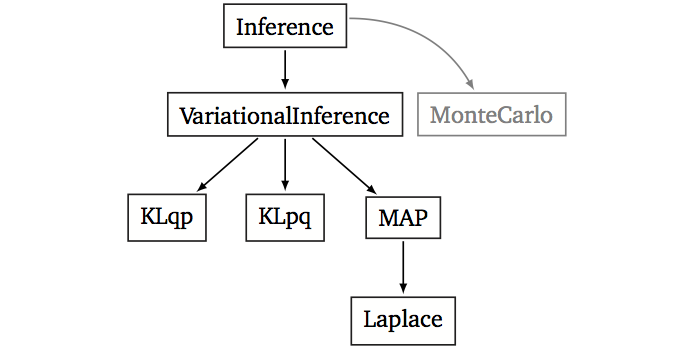
\includegraphics[width=700px]{/images/inference_structure.png}
{\small\textit{Dependency graph of inference methods.
Nodes are classes in Edward and arrows represent class inheritance.}}

There is a base class \texttt{Inference}, from which all inference
methods are derived from.

\begin{lstlisting}[language=Python]
class Inference(object):
  """Base class for Edward inference methods.
  """
  def __init__(self, latent_vars, data=None, model_wrapper=None):
    ...
\end{lstlisting}

It takes as input the set of latent variables to infer and a dataset. Optionally, if the user uses an external language to specify the model, it takes as input a model wrapper \texttt{model_wrapper}.

Note that \texttt{Inference} says nothing about the class of models that an
algorithm must work with. One can build inference algorithms which are
tailored to a restricted class of models available in Edward (such as
differentiable models or conditionally conjugate models), or even
tailor it to a single model. The algorithm can raise an error if the
model is outside this class.

We organize inference under two paradigms:
\texttt{VariationalInference} and \texttt{MonteCarlo} (or more plainly,
optimization and sampling). These inherit from \texttt{Inference} and each
have their own default methods.

\begin{lstlisting}[language=Python]
class MonteCarlo(Inference):
  """Base class for Monte Carlo inference methods.
  """
  def __init__(latent_vars, data=None, model_wrapper=None):
    super(MonteCarlo, self).__init__(latent_vars, data, model_wrapper)

  ...


class VariationalInference(Inference):
  """Base class for variational inference methods.
  """
  def __init__(self, latent_vars, data=None, model_wrapper=None):
    super(VariationalInference, self).__init__(latent_vars, data, model_wrapper)

  ...
\end{lstlisting}

Let's look at \texttt{Inference}. The main method in
\texttt{Inference} is \texttt{run()}.

\begin{lstlisting}[language=Python]
class Inference(object):
  """Base class for Edward inference methods.
  """
  ...
  def run(self, *args, **kwargs):
    """A simple wrapper to run inference.
    """
    self.initialize(*args, **kwargs)
    for t in range(self.n_iter + 1):
      info_dict = self.update()
      self.print_progress(t, info_dict)

    self.finalize()

  ...
\end{lstlisting}

First, it calls \texttt{initialize()} to initialize the algorithm, such as
setting the number of iterations. Then, within a loop it calls
\texttt{update()} which runs one step of inference, as well as
\texttt{print_progress()} for displaying progress; finally, it
calls \texttt{finalize()} which runs the last steps as the inference
algorithm terminates.

For example, developing a new variational inference algorithm is as simple as
inheriting from \texttt{VariationalInference} or one of its derived
classes. \texttt{VariationalInference} implements many default methods such
as \texttt{initialize()} above. Let's go through snippets from this method.

\begin{lstlisting}[language=Python]
class VariationalInference(Inference):
  ...
  def initialize(self, ...):
    ...
    if n_minibatch is not None ...
      ...
      slices = tf.train.slice_input_producer(values)
      batches = tf.train.batch(slices, n_minibatch,
                               num_threads=multiprocessing.cpu_count())
      ...
      self.data = {key: value for key, value in
                   zip(six.iterkeys(self.data), batches)}
    ...
    loss = self.build_loss()
    ...
    optimizer = tf.train.AdamOptimizer(learning_rate)
    self.train = optimizer.minimize(loss, ...)
\end{lstlisting}

Three code snippets are highlighted in \texttt{initialize()}: the first
enables batch training with an argument \texttt{n_minibatch} for the batch
size; the second defines the loss function, building TensorFlow's
computational graph; the third sets up an optimizer to minimize the
loss. These three snippets are applicable to all of variational
inference, and are thus useful defaults for any derived class.

For examples of inference algorithms built in Edward, see the inference
\href{/tutorials/}{tutorials}. It can also be useful to simply look at
the
\href{https://github.com/blei-lab/edward/tree/master/edward/inferences}
{source code}.

{{autogenerated}}
